\title{Data Collection: The Simple Pendulum}
\author{An Introduction to Physics through Experiments}
\date{}

\maketitle

\section{Objectives}

\begin{enumerate}
    \item To understand basic data collection, representation, and interpretation.
    \item To observe the variation of the time period of a simple pendulum with different parameters.
\end{enumerate}

\section{Introduction}

In this preliminary experiment you will be exposed to the ideas of measurement, data collection, and elementary data interpretation using the simple pendulum. 

\subsection{Data Collection}

\subsubsection{Raw-Data Tables}

In this laboratory you will be observing physical phenomena that are relatively well understood. In general, you will be asked to either verify certain formulae or to extract the value of certain physical quantities from them. As a result, you would usually have an \textbf{independent variable} that you will change over the course of collecting data, and a \textbf{dependent variable} which you will \textit{measure}. The data that you will take will have to be taken systematically, in order for you to make full use of it. As a result, it is imperative that you learn to tabulate your raw data well, so that you do not run into trouble later.

You will need a lab (auxiliary) notebook within which you will take your readings. It is essential that none of these readings be changed; if you have noted down something wrong, strike it out, and write down the correct value. However, it is essential to have a record of all the data you have taken. Remember: this does not need to be neat, only understandable to \textbf{you}. The TA or course instructor will have to initial your data. Do not underestimate the temptation to change your data: never discount points unless you have adequate reason to do so, and \textbf{never} change the value of a reading so that it fits a trend that you imagine is the `right' one.

There is no strict `right' way to tabulate data. However, there are several wrong ways. Here is a simple example: 

\begin{table}[!htb]
\centering
\begin{tabular}{|C{4cm}|C{2cm}|C{2cm}|C{2cm}|C{4cm}|}
\hline
\rowcolor{Gray}
\textbf{Independent Variable {\color{gray}(unit)}} & \multicolumn{3}{|c|}{\textbf{Dependent Variable {\color{gray}(unit)}}} &\textbf{Derived Quantity {\color{gray}(unit)}} \\ \hline
{} & Trial 1 & Trial 2 & Trial 3 & {} \\
\hline
{} & {} & {} & {} & {} \\
\hline
{} & {} & {} & {} & {} \\
\hline
{} & {} & {} & {} & {} \\
 \hline
\end{tabular}
\caption{Sample data table}
\label{sampledata}
\end{table}

Spend some time deciding what data table to draw before beginning your experiment: it will help you decide what data to take.

\subsubsection{``How many readings should I take?''}

This is the question we hear the most often. The answer is of course that \textbf{it depends}. It certainly depends on the experimental setup, and it depends on the different types of uncertainties present in each measurement.

While some scientific measurements are exact\footnote{Counting the number of parents you have, for example.}, others -- such as the sorts of measurements you will be doing in this lab -- are not. When we make a measurement, we generally assume that some exact or true value exists based on how we define what is being measured. We attempt to find this quantity as best we can, with the available resources. 

You will notice that you obtain slightly different results on making multiple measurements of the same quantity. We will deal with this in great detail in the {\color{red}Error Analysis} section, but for now you may imagine that these are a result of random fluctuations about the `true' value. One way to increase your confidence in experimental data is to repeat the same measurement many times. If the errors are truly random, then there should be just as many \textit{above} the true value as \textit{below}. Thus, when you average your answer, you should get a more accurate answer.

For example, one way to estimate the amount of time it takes something to happen is to simply time it once with a stopwatch. However, this would involve random errors due to -- among other things -- your reaction time. You can decrease the uncertainty in this estimate by making this same measurement multiple times and taking the average. The more measurements you take, the better your estimate will be\footnote{Provided there is no problem with the clock! We will speak in detail of such systematic errors later.}.

Thus, before you decide how many readings you wish to take, you need to decide \textbf{what uncertainty it is you are trying to eliminate}. Here is a simple example of how to think about it in the experiment at hand, timing a simple pendulum:

\begin{enumerate}
    \item Let us assume the predominant uncertainty in the time period comes from human error: i.e., the fraction of time between the pendulum beginning an oscillation, and you starting the stopwatch.
    
    \item It turns out that this is roughly 0.3 seconds\footnote{Think of a way to estimate this.}. In other words, timing a pendulum that takes one second to oscillate would have an uncertainty of roughly 0.6 seconds\footnote{0.3s when you start the stopwatch, and 0.3s when you stop it.}! 
    
    \item You would like to reduce the effect this uncertainty has on the measurement, and so \textbf{one} oscillation is certainly not enough. What about 10? The total time of measurement will now be 10 seconds. However, the total uncertainty will \textit{still} be 0.6 seconds, since you're still only starting and stopping the stopwatch one time! 
    
    \item To find the time period, you would just divide by the number of oscillations (a fixed number that you know with absolute certainty), and this will cause the error to be divided by that number as well! Thus, you have an estimate of the time period, to within 0.06 seconds!
\end{enumerate}

\begin{question}
\paragraph{Question:} Since this is true, can you explain why taking the time period for a 1000 oscillations may not give you an answer that is much more accurate than 100 oscillations? ~\\

\paragraph{Question:} If you don't know what the predominant source of uncertainty is, how could you begin to estimate how uncertain your readings are?
\end{question}

\subsection{Data Representation}

Your performance in the lab will be judged almost exclusively through the reports of the work that you have done. You may have exhibited great ingenuity while collecting data or performing an experiment, but if that is not reflected in your final submission for the experiment, there is no way for us to grade you on it.

\subsubsection{Report}

Your lab report is as much an opportunity to show the instructor what you have learnt as it is to practice for composing professional technical reports after your graduation. Here are some things to keep in mind that will help you out when your report is graded.

Make your lab report \textbf{clear} and \textbf{easy to follow}. A common mistake students make is to write extremely long and elaborate reports that convey very little. We are not looking for pages and pages of writing; in fact, from experience, we have seen that the best reports are usually \textbf{short}. Just make sure that someone who hasn't done the lab can understand what you did and how you did it. It is your job to decide what is relevant and what isn't. This is good training for the future. 

\begin{imp}
Your lab report may be written by hand, on Microsoft Word, or using \LaTeX. Of these options, we suggest you begin using \LaTeX\, as soon as possible: it makes your work look professional, and learning to use it is good practice.
\end{imp}

\textbf{Data does not lie.} Contrary to popular opinion, grades are not assigned on how close the value obtained agrees with the ``correct'' one. If you are supposed to verify a law of nature, and you end up disproving it, that's fine, provided that you say that you disprove it. If however you cannot verify it, but say that you can, we can only assume that you didn't understand the experiment. If your results are completely different from established values, then you have probably measured or calculated something incorrectly. 

\begin{imp}
The lab report should contain \textbf{all} the information required for someone else to reproduce your experiment \textbf{and} its results, especially if your value deviates significantly from the agreed value; we should be able to trace back exactly what you did wrong.~\\

\textbf{A wrong answer with a clear path as to how you got there is worth significantly more than a right answer that appears unjustified or out of nowhere. }
\end{imp}

The handouts contain questions about the experiment are scattered around the manual. Make sure you answer them as you write your report; these questions are included at critical points to check your comprehension, and the answers often provide ideas of what to include in a good report. 

\begin{imp}
Spend some time thinking about the format of your lab report. We don't expect something publishable in Physical Review Letters, but on the other hand, we don't expect four pages of stream-of-consciousness writing either.
\end{imp}

\subsubsection{Figures, Graphs, and Tables}

Figures, Graphs, and Tables have a required standard of presentation, usually much higher than those you might put in your auxiliary book. If possible, have any tables and figures at the top and/or bottom of a page, and do not wrap text around figures or tables.

\begin{imp}
In general, you may use any software for data analysis. Beginners will usually prefer to use Microsoft Excel or Google Sheets. However, as you progress, it is \textbf{very strongly} advised that you use this lab to learn how to do very elementary plotting and data analysis using Python and Jupyter Notebook.
\end{imp}

\paragraph{Figures:} 
\begin{enumerate}
    \item The figures you will include in your lab report will usually be descriptions of the apparatus or circuit diagrams. 
    \item In general, they should be well marked and labelled and you should be able to refer to them through the report to better explain what you've done. 
    \item All figures should have a label (such as `Figure 1:' or `Fig.1:') at the start of a caption explaining what they describe. 
    \item Captions should be short and sufficiently informative so that anyone with some knowledge of the experiment will understand what it represents without having to refer to your report.
\end{enumerate}

\paragraph{Graphs:}
\begin{enumerate}
    \item Your graphs should be easy to read and clearly show all key features.
    \item Graphs are figures, and should therefore have a figure number at the start of their caption (`Fig.1:', not `Graph 1:').
    \item Consider whether various results can be combined into a single graph.
    \item Here are some things your graph \textbf{must} have:
    
    \begin{enumerate}
        \item Labelled axes with units,
        \item Error bars, indicating the uncertainty with which you know the location of the point,
        \item A white background,
        \item Sensible maximum and minimum values so that most of the space is filled by the graph.
    \end{enumerate}
    
    \item Your graph \textbf{does not} need to have:
    
    \begin{enumerate}
        \item A title: all the information about the graph should be in the caption,
        \item Grid-marks or a border,
        \item Legends (unless the graph cannot be understood without one): this information would preferably also go into the caption.
    \end{enumerate}

\end{enumerate}


\paragraph{Tables:}

\begin{enumerate}
    \item Like figures, Tables should be labelled and have a caption. However, they are \textbf{not} figures, but should instead be labelled `Table 1:', etc.
    \item All the entries, including the headings, should fit comfortably in the width or height of the columns or rows; long headings should be avoided. 
    \item The headings of the columns should include the \textbf{units} of the measurement. The readings themselves should not have units.
    \item Include the uncertainties in every reading.
    \item Make sure the rows and columns are the same size throughout the table.
\end{enumerate}

\begin{imp}
Don’t include tables of data when the information is adequately given in a graph or by a few words of text; this is redundant and wasteful of space. 
\end{imp}

\subsection{Data Interpretation}

The last step in your report is an \textbf{analysis} of your data. Usually, this is something that you can get from your graphs. Throughout this course you will be asked to plot graphs and to extract the relevant information from them. In general, this is something that is better learnt by doing rather than by reading.  Once a regression line has been found, the equation must be interpreted in terms of the context of the situation being analysed.

In general, it is good practice to always plot \textbf{linear} graphs whenever possible. In certain cases, the relationships between physical quantities are linear, and this is easy: for example, if a ball is dropped from rest from some height, its \textbf{velocity} $v$ varies as

\begin{equation*}
    v = g t
\end{equation*}

Plotting $v$ against $t$ will give you a \textbf{linear} graph whose slope is the acceleration due to gravity. However, such a variation is not always guaranteed for all physical quantities. For example, the \textbf{position} $S$ of the same ball varies as

\begin{equation*}
    S = \frac{1}{2} g t^2
\end{equation*}

which is a \textit{quadratic} relationship. In some cases, you might be tempted to plot $S$ as a function of $t$ and fit a quadratic curve. In general, it is better to plot a graph between $S$ and $t^2$. These two quantities exhibit a linear relationship which is easier to fit, and whose slope gives you $g/2$.

One reason for this is because when you have a very small number of points, different polynomials may appear to fit it equally well.


\section{Theory: The Simple Pendulum}

The simple pendulum is a point mass suspended from a string of negligible mass attached to a pivot point, as shown in Figure (\ref{simple}). 

\begin{figure}[!htb]
    \centering
    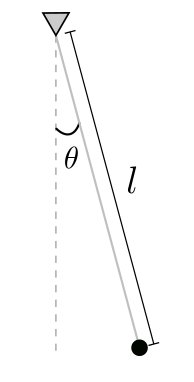
\includegraphics[scale=0.5]{figs/simplependulum.png}
    \caption{The Simple Pendulum}
    \label{simple}
\end{figure}

If a pendulum is set in motion so that is swings back and forth, its motion will be periodic. The time that it takes to make one complete oscillation is defined as the \textbf{time period} $T$ of the pendulum. Most of you will probably recognise the following formula for $T$: 

\begin{equation}
    T = 2 \pi \sqrt{\frac{l}{g}} 
    \label{TimeP}
\end{equation}

where $l$ is the length of the pendulum from its fixed point, and $g$ is the acceleration due to gravity. Not so many of you, however, will realise that this is only true for \textbf{small displacements} around the equilibrium position. In general, when the pendulum is displaced from its equilibrium position, it experiences a restoring force $m g \sin\theta$. The differential equation describing its motion can be obtained from Newton's Second Law  $m\vb{a} = \vb{F}$.

\begin{equation}
    m l \dv[2]{\theta}{t} = - m g \sin\theta
\end{equation}

This is a difficult differential equation to solve. In the approximation that the angle $\theta$ is very small, we can replace $\sin\theta \approx \theta$, and we are left with the following differential equation:

\begin{equation}
    \dv[2]{\theta}{t} + \frac{g}{l} \theta = 0
\end{equation}

It is in this approximation that the simple pendulum is a \textbf{simple harmonic oscillator}, a very important model that you will not stop seeing the end of. In general, a quantity $Q$ is considered observe simple harmonic variation with respect to some parameter $t$ (not necessarily time) if it satisfies the following differential equation:

\begin{equation*}
    \dv[2]{Q}{t} + \omega_0^2 Q = 0
\end{equation*}

where $\omega_0$ is the time period of the oscillation, and is related to the time period of the oscillation through 

\begin{equation*}
    T = \frac{2\pi}{\omega_0}
\end{equation*}

Comparing, you should see that in our case, $$\omega_0 = \sqrt{\frac{g}{l}}$$ and $$T = 2\pi \sqrt{\frac{l}{g}}$$

Thus, it should be clear that it is only when the amplitude is \textbf{small} that the time period follows this equation, since it is only then when you can approximate $\sin\theta$ with $\theta$.

In this introductory experiment you will begin by verifying the above formula for the time period for small angles. You will then attempt to explore any variation of the time period with angle.

\section{Apparatus}

\begin{enumerate}
    \item Metallic bobs of different materials
    \item A length of string
    \item A cork with a slit
    \item A retort stand with attached protractor
\end{enumerate}

\section{Suggested Procedure}

\begin{question} 
\paragraph{Question:} Which are the different physical quantities in this problem that can be varied to potentially change the time period\footnote{\textbf{Warning!} Do not use Equation (\ref{TimeP}) to answer this: we've already seen that that only works under certain special cases}?
\end{question}

\subsection{Part A}

In this part of the experiment you will design a simple experiment to determine the variation of the time period with the mass of the bob.

\begin{enumerate}
    \item Begin by deciding which variables you need to fix, and which variables you will change.
    
    \item Draw out an appropriate table in your auxiliary notebooks. Mark out any important details that would help you remember what you've done when you re-read this. Remember to state not only what you have changed, but also what you have kept \textit{fixed}.
    
    \item Decide on the \textbf{number} of readings you will take. When you have arrived at a number, try to \textit{justify} it.
    
    \item Perform the necessary experiment, varying the relevant parameter. Note down your data.
    
    \item Plot an appropriate graph that accurately depicts your results.
\end{enumerate}

\begin{question}
\paragraph{Question:} What graph would be the best to plot? Why? ~\\

\paragraph{Question:} What is your conclusion? How confident are you of this conclusion?
\end{question}


\subsection{Part B}

In this part of the experiment you will design a simple experiment to determine the variation of the time period with the length of the string from the pivot to the centre of mass of the bob.

\begin{enumerate}
    \item Begin by deciding which variables you need to fix, and which variables you will change.
    
    \item Draw out an appropriate table in your auxiliary notebooks. Mark out any important details that would help you remember what you've done when you re-read this. Remember to state not only what you have changed, but also what you have kept \textit{fixed}.
    
    \item Decide on the \textbf{number} of readings you will take. When you have arrived at a number, try to \textit{justify} it.
    
    \item Perform the necessary experiment, varying the relevant parameter. Note down your data.
    
    \item Plot an appropriate graph that accurately depicts your results.
\end{enumerate}


\begin{question}
\paragraph{Question:} What graph would be the best to plot? Why? ~\\

\paragraph{Question:} What is your conclusion? How confident are you of this conclusion?
\end{question}

\subsection{Part C}

In this part of the experiment you will design a simple experiment to determine the variation of the time period with the angle of release of the bob.

\begin{enumerate}
    \item Begin by deciding which variables you need to fix, and which variables you will change.
    
    \item Draw out an appropriate table in your auxiliary notebooks. Mark out any important details that would help you remember what you've done when you re-read this. Remember to state not only what you have changed, but also what you have kept \textit{fixed}.
    
    \item Decide on the \textbf{number} of readings you will take. When you have arrived at a number, try to \textit{justify} it.
    
    \item Perform the necessary experiment, varying the relevant parameter. Note down your data.
    
    \item Plot an appropriate graph that accurately depicts your results.
\end{enumerate}


\begin{question}
\paragraph{Question:} What graph would be the best to plot? Why? ~\\

\paragraph{Question:} What is your conclusion? How confident are you of this conclusion?
\end{question}

\paragraph{Note:} The repetition is -- of course -- intentional. We have found that students usually jump through these steps and -- as a result -- spend much of their time painstakingly collecting data that is of little or no use. It is essential that you spend some time deciding what exactly you want to collect, and how best you will represent it, before actually spending any time with the apparatus.



\section{Questions}

\begin{question}
\paragraph{Question:} What would be the effect -- if any -- of changing the \textbf{shape} of the bob on the time period? Justify your answer.
\end{question}